\documentclass{article}
\usepackage[utf8]{inputenc}
\usepackage{graphicx}
\graphicspath{{C:/Users/mech_engg_swag/Pictures/}}

\title{Variation of Error vs degree q keeping number of elements constant}
\author{Parth Thakkar}
\date{February 2018}

\begin{document}


\section*{Variation of Error vs degree q keeping number of elements constant}
An attempt was made to study the variation in error with increase in highest degree of Legendre polynomials. Thus, the function sin(x) was chosen. In order to investigate whether the error followed a trend like $c^{-q}$, we plotted log$\big[max(||E||_{2})\big]$ vs log(q) where E is the error and q is the highest degree of polynomials. This was done for total number of intervals = 5,6,7,8,9 and 10.
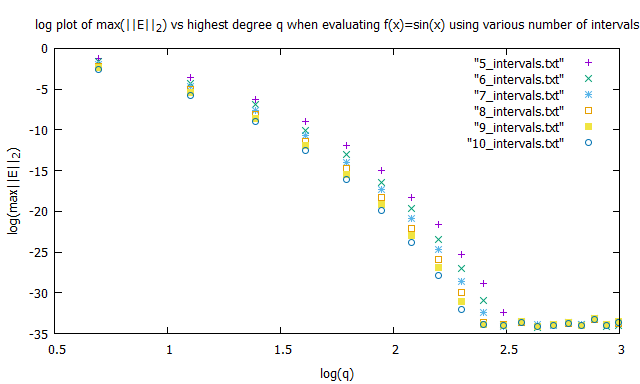
\includegraphics[scale=0.5]{hw3.png}

Thus we can see that we almost get a straight line with negative slope (starting with q=4) upto a certain value of q on the log-log plot. This means that the error does obey the law $E=c^{-q}$. After a certain value, the error is nearly constant, i.e. the value of log$\big[max(||E||_{2})\big]$ goes down to -35. This is because the error E=exp(-35) is of the order of $10^{-16}$, which is machine precision, i.e. it is beyond measure by our computers which work on double precision.
\end{document}
